\documentclass{article}
\input{new_commands}

% if you need to pass options to natbib, use, e.g.:
\PassOptionsToPackage{numbers, sort, compress}{natbib}
% before loading neurips_2024


% ready for submission
%\usepackage{neurips_2024}


% to compile a preprint version, e.g., for submission to arXiv, add add the
% [preprint] option:
\usepackage[preprint]{neurips_2024}


% to compile a camera-ready version, add the [final] option, e.g.:
%     \usepackage[final]{neurips_2024}


% to avoid loading the natbib package, add option nonatbib:
%    \usepackage[nonatbib]{neurips_2024}


\usepackage[utf8]{inputenc} % allow utf-8 input
\usepackage[T1]{fontenc}    % use 8-bit T1 fonts
\usepackage{hyperref}       % hyperlinks
\usepackage{url}            % simple URL typesetting
\usepackage{booktabs}       % professional-quality tables
\usepackage{amsfonts}       % blackboard math symbols
\usepackage{nicefrac}       % compact symbols for 1/2, etc.
\usepackage{microtype}      % microtypography
\usepackage{xcolor}         % colors

%%%

\usepackage{subcaption}
\usepackage{graphicx}
\usepackage{multirow}
\usepackage{amsmath,amssymb,amsfonts}
\usepackage{amsthm}
\usepackage{mathrsfs}
\usepackage{xcolor}
\usepackage{textcomp}
\usepackage{manyfoot}
\usepackage{booktabs}
\usepackage{algorithm}
\usepackage{algorithmicx}
\usepackage{algpseudocode}
\usepackage{listings}

\newtheorem{theorem}{Theorem} % continuous numbers
%%\newtheorem{theorem}{Theorem}[section] % sectionwise numbers
%% optional argument [theorem] produces theorem numbering sequence instead of independent numbers for Proposition
\newtheorem{proposition}[theorem]{Proposition}% 
\newtheorem{lemma}{Lemma}% 
%%\newtheorem{proposition}{Proposition} % to get separate numbers for theorem and proposition etc.

\newtheorem{example}{Example}
\newtheorem{remark}{Remark}

\newtheorem{definition}{Definition}
\newtheorem{assumption}{Assumption}

%%%


\title{Robust Convergence of Loss Landscapes through Distributional Averaging}


% The \author macro works with any number of authors. There are two commands
% used to separate the names and addresses of multiple authors: \And and \AND.
%
% Using \And between authors leaves it to LaTeX to determine where to break the
% lines. Using \AND forces a line break at that point. So, if LaTeX puts 3 of 4
% authors names on the first line, and the last on the second line, try using
% \AND instead of \And before the third author name.


\author{
  Nikita Kiselev\\
  MIPT\\
  Moscow, Russia\\
  \texttt{kiselev.ns@phystech.edu}\\
  \And
  Vladislav Meshkov\\
  MIPT\\
  Moscow, Russia\\
  \texttt{meshkov.vs@phystech.edu}\\
  \And
  Andrey Grabovoy\\
  MIPT\\
  Moscow, Russia\\
  \texttt{grabovoy.av@phystech.edu}\\
}


\begin{document}


\maketitle

\begin{abstract}
Understanding how a neural network’s loss landscape evolves with dataset size is essential for identifying sufficient training data. 
Prior analyses of this problem have typically been local, focusing on second-order expansions around a single optimum and bounding convergence through Hessian properties. 
While such studies clarify convergence rates, they provide only a pointwise view of stability. 
In this paper, we extend the framework to a distributional paradigm. 
Instead of analyzing convergence at one optimum, we evaluate it in expectation over a parameter distribution. 
This approach captures how entire neighborhoods of the loss landscape stabilize as additional samples are added. 
We focus on Gaussian distributions centered at local minima and employ Monte Carlo sampling to estimate convergence in practice. 
Theoretically, we show that distributional convergence exhibits the same asymptotic rate as the local case, while offering a more robust picture of stability. 
Empirical studies on image classification tasks confirm these predictions and highlight how architectural choices such as normalization, dropout, and network depth influence convergence. 
Our results broaden local convergence analyses into a distributional setting, providing stronger guarantees and practical tools for characterizing dataset sufficiency.
\end{abstract}


\textbf{Keywords:} Neural networks, Loss landscape, Convergence, Gaussian sampling, Monte Carlo estimation, Dataset size.

\section{Introduction}\label{sec:intro}

\begin{figure}[ht]
    \centering
    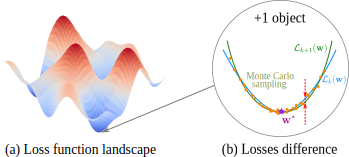
\includegraphics[width=0.65\linewidth]{losses_difference_monte_carlo.pdf}
    \caption{\textbf{Overview of our observations.} Part (a) shows the loss function landscape, which is a surface in the parameters space. Part (b) shows the losses difference. We propose the $\Delta_k$ metric, which in practice is a Monte~Carlo estimation of a squared losses difference over a Gaussian distribution near the local minima.}
    \label{fig:overview}
\end{figure}

Neural networks achieve strong performance across domains such as image classification, language modeling, and generative modeling. 
As datasets and models scale, accuracy improves but at growing computational cost. 
This raises a fundamental question: \emph{how large must the dataset be before additional samples cease to meaningfully alter the optimization landscape?} 
Answering this is central both for theoretical understanding of generalization and for practical training decisions.

One way to study this problem is through the geometry of the loss landscape. 
Curvature near minima reflects generalization, stability, and optimization dynamics \cite{neyshabur2017exploringgeneralizationdeeplearning, fort2019emergentpropertieslocalgeometry}. 
Flatter minima are linked to robustness, while sharper ones often overfit \cite{hochreiter1997flatminima}. 
The Hessian, encoding second-order curvature, is central in such analyses \cite{sagun2017eigenvalueshessiandeeplearning,ghorbani2019investigation}. 
Yet little is known about how these properties evolve with increasing dataset size.

In earlier work we analyzed \emph{loss landscape convergence with sample size} \cite{kiselev2024unraveling}. 
Using second-order Taylor expansions at local optima, we showed that the difference between losses trained on \(k\) and \(k+1\) samples vanishes as \(k \to \infty\), with rates governed by the Hessian spectral norm. 
This clarified how local curvature stabilizes with more data, but remained a \emph{pointwise} view tied to a single optimum~\(\bw^*\).

Here we extend that analysis to a \emph{distributional} framework. 
Instead of one point, convergence is measured in expectation under a parameter distribution \(p(\bw)\). 
This captures the stability of neighborhoods around optima and allows Monte Carlo estimation in practice. 
Gaussian neighborhoods offer a natural choice: they probe surrounding curvature while remaining tractable.

We prove that distributional convergence matches the quadratic rate of the pointwise case, while providing a stronger notion of stability by averaging across directions. 
Experiments on image classification validate the theory and reveal how batch normalization, dropout, and depth influence convergence.

\textbf{Contributions.} Our contributions can be summarized as follows.
\begin{itemize}
    \item Generalization of pointwise convergence analyses to a distributional framework over arbitrary parameter distributions \(p(\bw)\).
    \item Introduction of Gaussian neighborhoods around local optima and a Monte Carlo estimator for convergence.
    \item Theoretical guarantees showing distributional convergence decays at the same asymptotic rate as the local case, but with greater robustness.
    \item Empirical evaluation across architectures, highlighting how normalization, dropout, and depth reshape landscape stability.
\end{itemize}

\textbf{Outline.} Section~\ref{sec:rw} reviews related work. Section~\ref{sec:prelim} introduces notation. Section~\ref{sec:method} presents the framework and analysis. Section~\ref{sec:exp} reports experiments. Section~\ref{sec:disc} discusses implications and Section~\ref{sec:concl} concludes.

\section{Related Work}\label{sec:rw}

\textbf{Geometry of neural network loss landscapes.}  
The geometry of neural network loss functions has been a central theme in deep learning theory. Early studies analyzed the abundance of local minima and saddle points in high-dimensional spaces \cite{choromanska2015losssurfacesmultilayernetworks}, and later works revealed connectivity of minima through nearly flat valleys \cite{garipov2018losssurfacesmodeconnectivity, draxler2019essentiallynobarriers, nguyen2017losssurfacedeepwide}. The flatness or sharpness of minima is often linked to generalization, with flatter regions associated with more robust solutions \cite{hochreiter1997flatminima, dinh2017sharpminimageneralizedeep}. Visualization approaches \cite{li2018visualizing} and analyses of double descent and training instabilities \cite{singh2022phenomenologydoubledescentfinitewidth, wang2023instabilitieslargelearningrate} further highlight how architectural choices, initialization, or optimization interact with the underlying geometry. More recent work has also examined landscape properties in transformers and vision models \cite{chen2022visiontransformersoutperformresnets, lee2024visualizinglosslandscapeselfsupervised}. These studies provide qualitative and structural insights into geometry, but do not directly address how landscapes converge with increasing dataset size.

\textbf{Hessian spectra and curvature analyses.}  
The Hessian matrix is a powerful tool for quantifying curvature and stability in trained networks. Empirical studies show that its spectrum typically consists of a large bulk near zero and a few outliers that capture informative directions \cite{sagun2017eigenvalueshessiandeeplearning,ghorbani2019investigation,papyan2019spectrumdeepnethessiansscale,papyan2020tracesclasscrossclassstructurepervade}. Outlier structure has been tied to class-level geometry \cite{papyan2019measurementsthreelevelhierarchicalstructure}, while random matrix and maximum-entropy models explain power-law tails \cite{pmlr-v70-pennington17a, xie2022powerlawhessianspectrumsdeep, liao2021hessianeigenspectrarealisticnonlinear}. Decomposition methods, such as Kronecker factorizations, provide scalable approximations and structural interpretations \cite{wu2022dissectinghessianunderstandingcommon, singh2021analyticinsightsstructurerank, singh2023hessianperspectivenatureconvolutional}. Beyond structural analysis, curvature has been directly connected to generalization and robustness \cite{fort2019emergentpropertieslocalgeometry, ju2023robustfinetuningdeepneural, nguyen2024agnosticsharpnessawareminimization, macdonald2023progressivesharpeningflatminima}. Our earlier studies also fall into this direction: in \cite{kiselev2024unraveling} we introduced a Hessian-based framework for analyzing convergence in fully connected networks, and in \cite{meshkov2024conv} extended it to convolutional architectures. However, most Hessian-based analyses remain local, focusing on pointwise curvature near minima rather than distributional stability across neighborhoods.

\textbf{Dataset size, stability, and scaling perspectives.}  
A complementary line of work investigates how dataset size affects both generalization and optimization. Empirically, larger datasets tend to produce flatter landscapes and more stable solutions \cite{wu2017towards}, while scaling law studies explore systematic trade-offs among model size, dataset size, and compute \cite{hoffmann2022training}. Algorithmic stability theory \cite{bousquet2002stability, elisseeff2005stability, hardt2016trainingsgd} provides generalization guarantees by bounding sensitivity to changes in the training set, offering a perspective closely related to our notion of landscape convergence. Connections to kernel regimes \cite{NEURIPS2018_5a4be1fa, Lee_2020} also motivate quadratic and distributional approximations.
Beyond these general perspectives, recent work has begun to study sample size determination directly. In particular, authors introduced several methods for linear models based on likelihood bootstrapping \cite{kiselev2025likelihood} and parameters posterior distributions proximity \cite{kiselev2025posterior}.
Yet despite this broad literature, the question of how loss landscapes themselves converge as dataset size increases has remained largely unexplored. Our contribution addresses this gap by formalizing convergence in expectation under parameter distributions, thereby connecting geometric insights from Hessian spectra with stability-style notions from learning theory.


\section{Preliminaries}\label{sec:prelim}

\subsection{Notation}
We denote a neural network with parameters $\mathbf{w} \in \mathbb{R}^N$ by $f_{\mathbf{w}}$.  
Let the training dataset be $\mathfrak{D} = \{(\mathbf{x}_i, \mathbf{y}_i)\}_{i=1}^D$ of size $D$, where $\mathbf{x}_i \in \mathcal{X}$ and $\mathbf{y}_i \in \mathcal{Y}$. For a subset $\mathfrak{D}_k = \{(\mathbf{x}_i, \mathbf{y}_i)\}_{i=1}^k$ with $k < D$, the empirical loss is
\[
    \mathcal{L}_k(\mathbf{w}) = \frac{1}{k} \sum_{i=1}^{k} \ell(f_{\mathbf{w}}(\mathbf{x}_i), \mathbf{y}_i) = \frac{1}{k}\sum_{i=1}^k \ell_i(\mathbf{w}),
\]
where $\ell_i(\mathbf{w})$ is the per-sample loss. The difference in empirical loss when adding the $(k+1)$-th example is
\[
    \mathcal{L}_{k+1}(\mathbf{w}) - \mathcal{L}_k(\mathbf{w}) = \frac{1}{k+1}\Big(\ell_{k+1}(\mathbf{w}) - \mathcal{L}_k(\mathbf{w})\Big).
\]

To quantify landscape change, we define the squared-difference criterion:
\[
    \Delta_{k+1} = \mathbb{E}_{p(\mathbf{w})}\Big[ \big( \mathcal{L}_{k+1}(\mathbf{w}) - \mathcal{L}_k(\mathbf{w}) \big)^2 \Big],
\]
where $p(\mathbf{w})$ is a weighting distribution over parameter space (e.g., Gaussian around a local minimum). Thus, in practice, $\Delta_{k+1}$ can be estimated via Monte Carlo:
\[
    \Delta_{k+1} \approx \frac{1}{B}\sum_{t=1}^B \big( \mathcal{L}_{k+1}(\mathbf{w}^{(t)}) - \mathcal{L}_k(\mathbf{w}^{(t)}) \big)^2, 
    \quad \mathbf{w}^{(t)} \sim p(\mathbf{w}).
\]

\subsection{Assumptions}
Our theoretical analysis relies on the following assumptions, standard in loss landscape studies:
\begin{assumption}[Smoothness]
Each per-sample loss $\ell_i(\mathbf{w})$ is twice continuously differentiable.  
\end{assumption}

\begin{assumption}[Existence of local minima]
For each $k$, there exists at least one local optimum $\mathbf{w}^*_k$ such that $\nabla \mathcal{L}_k(\mathbf{w}^*_k) = \mathbf{0}$.  
\end{assumption}

\begin{assumption}[Bounded Hessians]
The Hessians at local minima are bounded: 
\[
    \|\mathbf{H}_i(\mathbf{w}^*_k)\|_2 \leq M_{\mathbf{H}}, \quad \forall i, k,
\]
where $\mathbf{H}_i$ is the Hessian of $\ell_i$.  
\end{assumption}

\begin{assumption}[Sampling distribution]
Parameter vectors $\mathbf{w}$ for evaluating $\Delta_{k}$ are drawn from a distribution $p(\mathbf{w})$ with mean $\mathbf{m}$ and covariance $\boldsymbol{\Sigma}$. A typical choice is Gaussian: $p(\mathbf{w}) = \mathcal{N}(\mathbf{m}, \sigma^2 \mathbf{I})$.  
\end{assumption}

These assumptions allow us to characterize how empirical loss surfaces converge as the dataset size increases, and to derive rates for $\Delta_k$ in terms of spectral and Frobenius norm bounds on Hessian differences.

\section{Method}\label{sec:method}

We now develop a formal analysis of loss landscape convergence. Our goal is to characterize how the difference between empirical losses $\mathcal{L}_k$ and $\mathcal{L}_{k+1}$ evolves as the dataset size increases, and to provide explicit convergence rates for the squared difference criterion $\Delta_{k+1}$. 
Unlike previous work that focused on a single optimum, we extend the framework by integrating over a distribution of parameters. This enables a more robust notion of convergence, since it captures how neighborhoods of optima evolve rather than just isolated points.

\subsection{Loss landscape change near local optima}
Let $\mathbf{w}^*_k$ denote a local minimum of $\mathcal{L}_k$, i.e. $\nabla \mathcal{L}_k(\mathbf{w}^*_k) = 0$. A second-order Taylor expansion around $\mathbf{w}^*_k$ gives
\[
    \mathcal{L}_k(\mathbf{w}) \approx \mathcal{L}_k(\mathbf{w}^*_k) + \tfrac{1}{2}(\mathbf{w}-\mathbf{w}^*_k)^\top \mathbf{H}^{(k)}(\mathbf{w}^*_k)(\mathbf{w}-\mathbf{w}^*_k),
\]
with $\mathbf{H}^{(k)}(\mathbf{w}^*_k)$ denoting the Hessian of $\mathcal{L}_k$ at $\mathbf{w}^*_k$.  
Applying the same expansion for $\mathcal{L}_{k+1}$ and subtracting yields
\[
    \mathcal{L}_{k+1}(\mathbf{w}) - \mathcal{L}_k(\mathbf{w}) 
    \approx \mathcal{L}_{k+1}(\mathbf{w}^*_k) - \mathcal{L}_k(\mathbf{w}^*_k) 
    + \tfrac{1}{2}(\mathbf{w}-\mathbf{w}^*_k)^\top \mathbf{A}_k (\mathbf{w}-\mathbf{w}^*_k),
\]
where
\[
    \mathbf{A}_k = \mathbf{H}^{(k+1)}(\mathbf{w}^*_k) - \mathbf{H}^{(k)}(\mathbf{w}^*_k).
\]

This local expansion forms the foundation of earlier pointwise analyses. In our setting, however, it also serves as the starting point for distributional averaging: by substituting these expansions into $\Delta_{k+1}$, we capture how curvature fluctuations propagate under $p(\bw)$.


\subsection{Squared difference criterion}
The convergence measure defined in Section~\ref{sec:prelim} can thus be expressed as
\[
    \Delta_{k+1} = \mathbb{E}_{p(\mathbf{w})}\Big[ \big( \mathcal{L}_{k+1}(\mathbf{w}) - \mathcal{L}_k(\mathbf{w}) \big)^2 \Big].
\]
Expanding the square and using standard variance decomposition gives
\[
    \Delta_{k+1} = \mathbb{D}_{p(\mathbf{w})}\big[ \mathcal{L}_{k+1}(\mathbf{w}) - \mathcal{L}_k(\mathbf{w}) \big] 
    + \Big(\mathbb{E}_{p(\mathbf{w})}[ \mathcal{L}_{k+1}(\mathbf{w}) - \mathcal{L}_k(\mathbf{w}) ]\Big)^2.
\]

For a Gaussian sampling distribution $p(\mathbf{w}) = \mathcal{N}(\mathbf{w}^*_k, \sigma^2\mathbf{I})$ centered at $\mathbf{w}^*_k$, and under the natural assumption that $\mathcal{L}_{k+1}(\mathbf{w}^*_k) \approx \mathcal{L}_k(\mathbf{w}^*_k)$, the mean term vanishes. We then obtain the simplified form
\[
    \Delta_{k+1} = \frac{\sigma^4}{4}\Big(\mathrm{Tr}^2(\mathbf{A}_k) + 2\mathrm{Tr}(\mathbf{A}_k^2)\Big).
\]

The Monte Carlo estimator provides a scalable way to approximate this expectation in practice, making it possible to track $\Delta_k$ across architectures and datasets. Importantly, this aligns the theory with empirical visualization tools: we can evaluate $\Delta_k$ in the same neighborhoods where landscape plots are drawn.

\subsection{Bounding the trace terms}
The traces can be controlled by spectral properties of $\mathbf{A}_k$.  
By Cauchy–Schwarz,
\[
    \mathrm{Tr}(\mathbf{A}_k) \leq \sqrt{N}\,\|\mathbf{A}_k\|_F, 
    \qquad 
    \mathrm{Tr}(\mathbf{A}_k) \leq N \|\mathbf{A}_k\|_2,
\]
while
\[
    \mathrm{Tr}(\mathbf{A}_k^2) = \|\mathbf{A}_k\|_F^2 \leq N \|\mathbf{A}_k\|_2^2.
\]

Thus,
\[
    \mathrm{Tr}^2(\mathbf{A}_k) + 2\mathrm{Tr}(\mathbf{A}_k^2) \;\leq\; N^2 \|\mathbf{A}_k\|_2^2 + 2N \|\mathbf{A}_k\|_2^2.
\]

\begin{lemma}[Trace bound]
For any symmetric matrix $\mathbf{A}_k \in \mathbb{R}^{N \times N}$,
\[
    \mathrm{Tr}^2(\mathbf{A}_k) + 2\mathrm{Tr}(\mathbf{A}_k^2) \;\leq\; N(N+2)\|\mathbf{A}_k\|_2^2.
\]
\end{lemma}

This bound ensures that the distributional convergence measure remains controlled by well-understood spectral quantities, connecting our generalization directly back to Hessian-based analyses of prior work.

\subsection{Bounding the Hessian difference}
By construction,
\[
    \mathbf{A}_k = \frac{1}{k+1}\Big(\mathbf{H}_{k+1}(\mathbf{w}^*_k) - \frac{1}{k}\sum_{i=1}^k \mathbf{H}_i(\mathbf{w}^*_k)\Big).
\]
If $\|\mathbf{H}_i(\mathbf{w}^*_k)\|_2 \leq M_{\mathbf{H}}$ for all $i$, then
\[
    \|\mathbf{A}_k\|_2^2 \leq \frac{2M_{\mathbf{H}}^2}{(k+1)^2}.
\]

Intuitively, this expresses that as the dataset grows, the variability in curvature introduced by adding one new example becomes negligible, which formalizes the geometric notion of ``sample sufficiency.''

\subsection{Convergence rate}
Substituting the above bounds into the expression for $\Delta_{k+1}$ yields
\[
    \Delta_{k+1} \leq \frac{\sigma^4}{4}\, N(N+2)\, \|\mathbf{A}_k\|_2^2 
    \leq \frac{\sigma^4 N(N+2) M_{\mathbf{H}}^2}{2(k+1)^2}.
\]

\begin{theorem}[Convergence rate of loss landscapes]
Under Assumptions 1–4, the squared difference between empirical loss landscapes at sample sizes $k$ and $k+1$ satisfies
\[
    \Delta_{k+1} = \mathcal{O}\Big(\frac{1}{(k+1)^2}\Big).
\]
Thus, as the dataset grows, loss landscapes converge quadratically fast in sample size.
\end{theorem}

This result shows that extending from pointwise to distributional averaging does not change the asymptotic convergence rate: both decay quadratically with dataset size. However, the distributional setting provides a much stronger guarantee, since it demonstrates that entire neighborhoods around minima stabilize, not just single points.

\section{Experiments}\label{sec:exp}

We now validate our theoretical framework through empirical studies. Our experiments address three main questions:  
(1) How does the loss landscape geometry evolve with architectural choices such as dropout, batch normalization, and network depth?  
(2) How does the proposed convergence measure $\Delta_k$ behave in practice?  
(3) Can $\Delta_k$ provide a geometric interpretation of sample size sufficiency analogous to scaling law studies?  

\subsection{Experimental Setup}
We use the CIFAR-10 dataset (50k training and 10k test images, 10 balanced classes). Networks are trained for classification with cross-entropy loss. Unless otherwise stated, optimization is performed with Adam (learning rate $3 \times 10^{-4}$, batch size 64).  

To visualize high-dimensional loss landscapes, we project onto 2D random subspaces. Specifically, given an optimum $\mathbf{w}^*$, we sample two random normalized directions $\mathbf{u}, \mathbf{v}$ with the same parameter norm ratios as $\mathbf{w}^*$, and evaluate
\[
    f(\alpha, \beta) = \mathcal{L}(\mathbf{w}^* + \alpha \mathbf{u} + \beta \mathbf{v}).
\]
This follows the common visualization protocol of \citet{li2018visualizing}.

\subsection{Effects of Dropout and Batch Normalization on the Loss Landscape}  
In the following experiments, 4-layer convolutional networks were trained with 64 channels in the hidden layers, a kernel size of 3, and ReLU activations. ReLU and batch normalization were added depending on the experiment.
Figure~\ref{fig:conv-dropout-batchnorm} demonstrates how the loss function landscape of convolutional networks changes when dropout and/or batch normalization are added to the neural network. Although the example is quite toy-like, it clearly illustrates the transformation of the landscape. Specifically, one can see that the introduction of batch normalization leads to a substantial ``narrowing'' of the landscape, while adding dropout afterward causes it to widen again.

\begin{figure}[h]
    \centering
    \includegraphics[width=0.3\linewidth]{loss_visualization/conv.png}
    \includegraphics[width=0.3\linewidth]{loss_visualization/conv_no_dropout.png}
    \includegraphics[width=0.3\linewidth]{loss_visualization/conv_no_bn_no_dropout.png}
    \caption{Convolutional networks (4 layers). \textbf{Left:} with dropout + batch norm, \textbf{center:} without dropout, \textbf{right:} without both. Batch normalization narrows the landscape, dropout widens it, while removing both produces unstable minima.}
    \label{fig:conv-dropout-batchnorm}
\end{figure}

The next experiments involved training a 4-layer fully connected neural network with 128-unit hidden layers using ReLU activations. Batch normalization and dropout were incorporated depending on the specific task configuration.
Figure~\ref{fig:fc-dropout-batchnorm} presents a similar experiment but with a fully connected network instead of a convolutional one, where the resulting loss landscape exhibits different properties. In particular, the landscape transforms less predictably and varies differently across different parameter space directions. When both batch normalization and dropout are applied simultaneously, the landscape becomes notably wider~--- an effect more pronounced than in convolutional networks.

\begin{figure}[h]
    \centering
    \includegraphics[width=0.3\linewidth]{loss_visualization/mlp.png}
    \includegraphics[width=0.3\linewidth]{loss_visualization/mlp_no_dropout.png}
    \includegraphics[width=0.3\linewidth]{loss_visualization/mlp_no_bn_no_dropout.png}
    \caption{Fully connected networks (4 hidden layers, 128 units). \textbf{Left:} with dropout + batch norm, \textbf{center:} without dropout, \textbf{right:} without both. Unlike convolutional models, the combination of dropout and batch norm produces the widest landscapes.}
    \label{fig:fc-dropout-batchnorm}
\end{figure}

\subsection{Loss Landscape Dynamics Near Optima with Varying Convolutional Blocks}\label{main:conv_layers_num}
The next three experiments involve training a convolutional neural network with ReLU activations and 64 channels in the hidden layers, while varying the number of layers.
Figure~\ref{fig:conv-depth} demonstrates how the loss landscape evolves in the vicinity of the optimum as the number of convolutional blocks changes. The visualization reveals that increasing network depth leads to a significantly wider landscape and more complex geometry. While shallow networks (2 layers) exhibit nearly parabolic shapes, deeper architectures produce more complex structure.

\begin{figure}[h]
    \centering
    \includegraphics[width=0.3\linewidth]{loss_visualization/conv_layers_num_2.png}
    \includegraphics[width=0.3\linewidth]{loss_visualization/conv_layers_num_4.png}
    \includegraphics[width=0.3\linewidth]{loss_visualization/conv_layers_num_6.png}
    \caption{This image shows the loss landscape of convolutional models with varying numbers of layers ($2 \rightarrow 4 \rightarrow 6$), illustrating how the loss landscape changes with increasing network depth.}
    \label{fig:conv-depth}
\end{figure}

\subsection{Delta calculation method hyperparameters influence}

This experiment employed a fully connected network with 4 hidden layers of 128 units each, ReLU activation, along with batch normalization and dropout.

In Figure~\ref{fig:k-deltak}, we observe how $\Delta_k$ depends on the parameter $\sigma$ in the distribution $p(\bw)$. Notably, the dependence is significant, indicating that this parameter strongly affects the locality of the estimated landscape change.

In the same figure (\textbf{right}), we observe the dependence on the dim used for landscape evaluation. Notably, the results exhibit high noise levels, suggesting this parameter likely does not require fine-tuning. Since visualization tests confirmed reproducibility across different random seeds, we subsequently use dim=2 for convenience. Figure~\ref{fig:integrated-squared-difference} demonstrates the variation of $(\cL_{k+1} - \cL_k)^2p(\bw)$ (the integrand quantity), for different values of $k$. Specifically, we observe that as $k$ increases while keeping $p(\bw)$ parameters constant, local behavior becomes increasingly dominant.

\begin{figure}[h]
    \centering
    \includegraphics[width=0.46\linewidth]{loss_visualization/delta_vis/compare_sigm.png}
    \includegraphics[width=0.46\linewidth]{loss_visualization/delta_vis/compare_dim.png}
    \caption{The \textbf{left} plot demonstrates how the estimated quantity varies with changes in the distribution parameter (specifically, the variance $\sigma^2$) of $p(w)$. The \textbf{right} plot shows its dependence on the number of random directions (dim).}
    \label{fig:k-deltak}
\end{figure}


\begin{figure}[h]
    \centering
    \begin{minipage}[h]{0.3\linewidth}
    \includegraphics[width=1\linewidth]{loss_visualization/vis_diff/diff_2_1.png}\subcaption[1]{$(\cL_1 - \cL_2)^2p(\bw)$}
    \end{minipage}
    \begin{minipage}[h]{0.3\linewidth}
    \includegraphics[width=1\linewidth]{loss_visualization/vis_diff/diff_50_51.png}
    \subcaption[2]{$(\cL_{50} - \cL_{49})^2p(\bw)$}
    \end{minipage}
    \begin{minipage}[h]{0.3\linewidth}
    \includegraphics[width=1\linewidth]{loss_visualization/vis_diff/diff_100_101.png}
    \subcaption[3]{$(\cL_{100} - \cL_{101})^2p(\bw)$}
    \end{minipage}
    \caption{This figure shows how the $\big(\cL_{k+1}(\bw) - \cL_{k}(\bw)\big)p(\bw)$ changes as the sample size used to estimate it varies.}
    \label{fig:integrated-squared-difference}
\end{figure}

\section{Discussion}\label{sec:disc}

Our results show that empirical loss landscapes converge quadratically fast with dataset size, as captured by the metric $\Delta_k$. 
The experiments confirm this trend: as $k$ increases, $(\mathcal{L}_{k+1} - \mathcal{L}_k)^2 p(\mathbf{w})$ smooths out and local fluctuations diminish. 
We now discuss the implications and boundaries of these findings.

\paragraph{Geometric notion of sample sufficiency.}  
Performance metrics such as accuracy or cross-entropy are standard proxies for dataset sufficiency. 
Our framework suggests a complementary, geometric criterion: once $\Delta_k$ falls below a threshold, the loss surface becomes stable enough that additional samples no longer significantly alter optimization geometry. 
This view connects data sizing to measurable landscape properties, offering a tool for reasoning about when a dataset is ``large enough.''

\paragraph{Impact of architectural choices.}  
We observed that architectural elements reshape convergence behavior. 
Batch normalization narrows valleys in convolutional networks, dropout widens them, and deeper models introduce more complex curvature patterns. 
In fully connected architectures, the interplay of dropout and normalization differs qualitatively. 
These findings highlight that convergence speed and stability are not solely functions of dataset size but also of design decisions, underlining the need to analyze architecture and data jointly.

\paragraph{Assumptions and limitations.}  
Our theoretical guarantees rely on quadratic approximations around local minima, Gaussian parameter distributions, and bounded Hessians. 
Real networks may violate these assumptions: multimodal loss landscapes and heavy-tailed curvature spectra are common, especially in large-scale transformers and language models. 
Furthermore, our experiments were confined to medium-scale image classification. 
Assessing whether distributional convergence persists in large architectures, alternative data modalities, and non-Gaussian parameter distributions remains an open challenge.

\section{Conclusion}\label{sec:concl}

We developed a distributional framework for studying loss landscape convergence, showing that neighborhoods around optima stabilize at the same quadratic rate as pointwise analyses. 
This provides a stronger and more practical notion of stability, with empirical confirmation across several architectures. 
Looking ahead, extending this framework to large-scale models, exploring non-Gaussian parameter distributions, and connecting convergence measures to generalization bounds represent promising directions for future work.


%%%%%%%%%%%%%%%%%%%%%%%%%%%%%%%%%%%%%%%%%%%%%%%%%%%%%%%%%%%%

\bibliographystyle{unsrtnat}
\bibliography{references}

%%%%%%%%%%%%%%%%%%%%%%%%%%%%%%%%%%%%%%%%%%%%%%%%%%%%%%%%%%%%

\newpage
\appendix
\section{Appendix: Proofs}\label{app:proofs}

\subsection{Proof of Lemma 1 (Trace bound)}
\begin{proof}
Let $\lambda_1, \dots, \lambda_N$ be the eigenvalues of the symmetric matrix $\mathbf{A}_k$. Then
\[
    \mathrm{Tr}(\mathbf{A}_k) = \sum_{i=1}^N \lambda_i,
    \qquad 
    \mathrm{Tr}(\mathbf{A}_k^2) = \sum_{i=1}^N \lambda_i^2.
\]
By Cauchy–Schwarz,
\[
    \Big(\sum_{i=1}^N \lambda_i\Big)^2 \leq N \sum_{i=1}^N \lambda_i^2.
\]
Thus,
\[
    \mathrm{Tr}^2(\mathbf{A}_k) + 2\mathrm{Tr}(\mathbf{A}_k^2) 
    \leq N \sum_{i=1}^N \lambda_i^2 + 2 \sum_{i=1}^N \lambda_i^2
    = (N+2)\sum_{i=1}^N \lambda_i^2.
\]
Finally, since $\max_i |\lambda_i| = \|\mathbf{A}_k\|_2$,
\[
    \sum_{i=1}^N \lambda_i^2 \leq N \|\mathbf{A}_k\|_2^2.
\]
Substituting gives
\[
    \mathrm{Tr}^2(\mathbf{A}_k) + 2\mathrm{Tr}(\mathbf{A}_k^2) \leq N(N+2)\|\mathbf{A}_k\|_2^2,
\]
which proves the claim.
\end{proof}

\subsection{Proof of Theorem 1 (Convergence rate of loss landscapes)}
\begin{proof}
From the derivation in Section~\ref{sec:method}, under Gaussian sampling around a local optimum $\mathbf{w}^*_k$ we have
\[
    \Delta_{k+1} = \frac{\sigma^4}{4}\Big(\mathrm{Tr}^2(\mathbf{A}_k) + 2\mathrm{Tr}(\mathbf{A}_k^2)\Big).
\]
Applying Lemma 1 gives
\[
    \Delta_{k+1} \leq \frac{\sigma^4}{4} \, N(N+2)\, \|\mathbf{A}_k\|_2^2.
\]
Now recall that
\[
    \mathbf{A}_k = \frac{1}{k+1}\left( \mathbf{H}_{k+1}(\mathbf{w}^*_k) - \frac{1}{k}\sum_{i=1}^k \mathbf{H}_i(\mathbf{w}^*_k)\right).
\]
By the bounded Hessian assumption $\|\mathbf{H}_i(\mathbf{w}^*_k)\|_2 \leq M_{\mathbf{H}}$ for all $i$, we have
\[
    \|\mathbf{A}_k\|_2 \leq \frac{1}{k+1}\Big(\|\mathbf{H}_{k+1}(\mathbf{w}^*_k)\|_2 + \frac{1}{k}\sum_{i=1}^k \|\mathbf{H}_i(\mathbf{w}^*_k)\|_2\Big) \leq \frac{2M_{\mathbf{H}}}{k+1}.
\]
Therefore,
\[
    \|\mathbf{A}_k\|_2^2 \leq \frac{4M_{\mathbf{H}}^2}{(k+1)^2}.
\]
Substituting into the upper bound for $\Delta_{k+1}$ yields
\[
    \Delta_{k+1} \leq \frac{\sigma^4}{4} \, N(N+2) \cdot \frac{4M_{\mathbf{H}}^2}{(k+1)^2} 
    = \frac{\sigma^4 N(N+2) M_{\mathbf{H}}^2}{(k+1)^2}.
\]
Thus,
\[
    \Delta_{k+1} = \mathcal{O}\Big(\frac{1}{(k+1)^2}\Big),
\]
which proves the theorem.
\end{proof}

\newpage
\section{Appendix: Experiments}\label{app:experiments}

In the main section, we analyzed landscapes at local optima obtained after fixed training epochs. 
Here we repeat the experiments but redefine $\bw^*$ as the \emph{validation-optimal parameters}, i.e., those corresponding to the best validation epoch (typically occurring early, between epochs 3–6). 
This adjustment provides a clearer view of generalization behavior, contrasting with the purely optimization-focused landscapes examined earlier.

\subsection{Loss landscapes near validation optima}\label{app:val_landscape}

\textbf{Setup.}  
We trained fully connected networks with 4 hidden layers of size 128 and batch size 64. 
Depending on the configuration, batch normalization and dropout blocks were inserted into each layer. 
For convolutional networks, we fixed 4 layers with 64 channels, kernel size 3, and padding 1.

\textbf{Results.}  
Figure~\ref{fig:fc-dropout-batchnorm-app} shows that in fully connected models, batch normalization produces narrower optima, while dropout widens the valleys. 
In convolutional models (Figure~\ref{fig:conv-dropout-batchnorm-app}), adding both batch normalization and dropout leads to sharper landscapes compared to vanilla networks. 
Figure~\ref{fig:conv-depth-app} compares networks of varying depth (2, 4, and 6 layers), revealing that deeper networks exhibit stronger boundary effects and more complex geometry at validation-optimal points.

\textbf{Takeaway.}  
The structure observed in the main experiments persists when evaluating at the best validation epoch, but landscapes are generally narrower and more sensitive at the boundaries, highlighting the connection between validation performance and curvature.

\subsection{Effects of hidden channel size}

\textbf{Setup.}  
We trained convolutional networks with varying numbers of hidden channels while keeping other hyperparameters fixed. 
Landscapes were evaluated within neighborhoods of equal norm to ensure comparability across models.

\textbf{Results.}  
As shown in Figure~\ref{fig:channels}, increasing the number of channels leads to progressively wider landscapes, with geometric deformation accelerating in deeper networks. 
This suggests that larger representational capacity amplifies curvature effects, though fixed-norm comparisons introduce dimensionality biases.

\textbf{Takeaway.}  
Channel count strongly influences curvature geometry at validation optima, reinforcing the role of network capacity in shaping landscape stability.

\begin{figure}[h]
    \centering
    \begin{minipage}[h]{0.32\linewidth}
    \includegraphics[width=1\linewidth]{loss_visualization/validation_landscape/no_bn_no_dropout_MLP_.png}\subcaption{vanilla FC}
    \end{minipage}
    \begin{minipage}[h]{0.32\linewidth}
    \includegraphics[width=1\linewidth]{loss_visualization/validation_landscape/no_dropout.png}
    \subcaption{FC with batch normalization}
    \end{minipage}
    \begin{minipage}[h]{0.32\linewidth}
    \includegraphics[width=1\linewidth]{loss_visualization/validation_landscape/MLP.png}
    \subcaption{FC with batch normalization and dropout}
    \end{minipage}
    \caption{Fully connected networks near validation-optimal parameters. Batch normalization narrows the optimum, dropout widens it.}
    \label{fig:fc-dropout-batchnorm-app}
\end{figure}

\begin{figure}[h]
    \centering
    \begin{minipage}[h]{0.32\linewidth}
    \includegraphics[width=1\linewidth]{loss_visualization/validation_landscape/val_landscape_conv/no_bn_no_dropout.png}\subcaption{vanilla ConvNet}
    \end{minipage}
    \begin{minipage}[h]{0.32\linewidth}
    \includegraphics[width=1\linewidth]{loss_visualization/validation_landscape/val_landscape_conv/no_dropout.png}
    \subcaption{ConvNet with batch normalization}
    \end{minipage}
    \begin{minipage}[h]{0.32\linewidth}
    \includegraphics[width=1\linewidth]{loss_visualization/validation_landscape/val_landscape_conv/conv.png}
    \subcaption{ConvNet with batch normalization and dropout}
    \end{minipage}
    \caption{Convolutional networks near validation-optimal parameters. Batch normalization and dropout sharpen the landscape relative to the vanilla case.}
    \label{fig:conv-dropout-batchnorm-app}
\end{figure}

\begin{figure}[h]
    \centering
    \begin{minipage}[h]{0.32\linewidth}
    \includegraphics[width=1\linewidth]{loss_visualization/validation_landscape/layers_num/layers_num=2.png}\subcaption{2 layers}
    \end{minipage}
    \begin{minipage}[h]{0.32\linewidth}
    \includegraphics[width=1\linewidth]{loss_visualization/validation_landscape/layers_num/layers_num=4.png}\subcaption{4 layers}
    \end{minipage}
    \begin{minipage}[h]{0.32\linewidth}
    \includegraphics[width=1\linewidth]{loss_visualization/validation_landscape/layers_num/layers_num=6.png}\subcaption{6 layers}
    \end{minipage}
    \caption{Loss landscapes of convolutional models with different depths near validation optima. Deeper networks exhibit stronger boundary effects and more complex curvature.}
    \label{fig:conv-depth-app}
\end{figure}

\begin{figure}[h]
    \centering
    \begin{minipage}[h]{0.3\linewidth}
    \includegraphics[width=1\linewidth]{loss_visualization/validation_landscape/hidden_channels/32.png}
    \subcaption{32 channels}
    \end{minipage}
    \hfill
    \begin{minipage}[h]{0.3\linewidth}
    \includegraphics[width=1\linewidth]{loss_visualization/validation_landscape/hidden_channels/64.png}
    \subcaption{64 channels}
    \end{minipage}
    \hfill
    \begin{minipage}[h]{0.3\linewidth}
    \includegraphics[width=1\linewidth]{loss_visualization/validation_landscape/hidden_channels/96.png}
    \subcaption{96 channels}
    \end{minipage}
    \begin{minipage}[h]{0.3\linewidth}
    \includegraphics[width=1\linewidth]{loss_visualization/validation_landscape/hidden_channels/128.png}
    \subcaption{128 channels}
    \end{minipage}
    \hfill
    \begin{minipage}[h]{0.3\linewidth}
    \includegraphics[width=1\linewidth]{loss_visualization/validation_landscape/hidden_channels/256.png}
    \subcaption{256 channels}
    \end{minipage}
    \caption{Effect of hidden channel size on loss landscapes at validation optima. Wider networks show progressively broader and more deformed landscapes.}
    \label{fig:channels}
\end{figure}



\end{document}